\subsection{Problem 2}%
\label{sec:problem_2}
Solve the following system of linear equations using the selected iterative solvers:
\begin{equation*}
  \systeme{x_1+x_2+x_3=1,x_1+x_2+2x_3=2,x_1+2x_2+2x_3=1}
\end{equation*}
Compare and discuss the computational costs with respect to convergence rates.
Start the iterations from $\matr{x}^{(0)}=\matr{0}$.
%%%%%%%%%%%%%%%%%%%%%%%%%%%%%%%%%%%%%%%%%%%%%%%%%%%%%%%%%%%%%%%%%%%%%%%%%%%%%%%
\subsubsection*{Mathematics}
%%%%%%%%%%%%%%%%%%%%%%%%%%%%%%%%%%%%%%%%%%%%%%%%%%%%%%%%%%%%%%%%%%%%%%%%%%%%%%%
First step that was taken before creating plots, convergence of methods has been checked.
\begin{itemize}
  \item Jacobi \\
  Calculated eigenvalues for this method are 
  \begin{equation*}
    \begin{bmatrix}
      0 \\
      0.5000 \\
      2.0000
    \end{bmatrix}
  \end{equation*}
  Calculated spectral radius for Jacobi method gives $\rho \approx 2$ which disqualifies function from further use.
  \item Gauss-Seidel \\ 
  Eigenvalues for calculating spectral radius are 
  \begin{equation*}
    \begin{bmatrix}
      -2.1091 \\
      0.6498 \\
      1.4593
    \end{bmatrix}
  \end{equation*}
  Resulting in spectral radus $ \rho = 2.1091 $ which doesn't meet the criteria. 
  \item SOR \\
  Optimal $\omega$ relaxation factor wasn't able to be computed.
  Iterative approach for solving this problem didn't find any solution that would get spectral radius within convergence range.
  \item Landweber \\
  First step of calculations would be obtaining resulting matrix of operation $\matr{A}^TA$ for eigenvalue decomposition
  \begin{equation*}
    \matr{A}^TA = 
    \begin{bmatrix}
      1 & 1 & 1 \\
      1 & 2 & 2 \\
      1 & 1 & 2
      \end{bmatrix} * 
      \begin{bmatrix}
        1 & 1 & 1 \\
        1 & 2 & 1 \\
        1 & 2 & 2
      \end{bmatrix} = 
      \begin{bmatrix}
          3 & 5 & 4 \\
          5 & 9 & 7 \\
          4 & 7 & 6
      \end{bmatrix}
  \end{equation*}
  Next step would be obtaining eigenvalues from calculated matrix 
  \begin{equation*}
    \left|\begin{matrix}
      -\lambda+3 & 5 & 4 \\
      5 & -\lambda+9 & 7 \\
      4 & 7 & -\lambda+6
      \end{matrix}=\right|
      = -\lambda^3 + 18\lambda^2 - 9\lambda + 1
  \end{equation*}
  calculated eigenvalues are: 
  \begin{multicols}{3}
    \begin{itemize}
      \item[$\circ$] $\lambda_1 \approx 0.1652 $
      \par
      \item[$\circ$] $\lambda_2 \approx 0.3462 $
      \par
      \item[$\circ$] $\lambda_3 \approx 17.4887 $
    \end{itemize}
  \end{multicols}
  With maximal value determined being $\lambda_3 \approx 17.4887$ we can calculate convergence criteria 
  \begin{equation*}
    2 * |\lambda_{max}(\matr{A}^T\matr{A})|^{-1} = 2 * 17.4887^{-1} \approx 0.1144
  \end{equation*}
  This results in range of converging $\alpha$ values as:
  \begin{equation*}
    0 < \alpha < 0.1144
  \end{equation*}
\end{itemize}

%%%%%%%%%%%%%%%%%%%%%%%%%%%%%%%%%%%%%%%%%%%%%%%%%%%%%%%%%%%%%%%%%%%%%%%%%%%%%%%
\subsubsection*{Solution}
%%%%%%%%%%%%%%%%%%%%%%%%%%%%%%%%%%%%%%%%%%%%%%%%%%%%%%%%%%%%%%%%%%%%%%%%%%%%%%%
Exact solution for this problem is 
\begin{equation*}
  x =
  \begin{bmatrix}
    1 \\
    -1 \\
    1
  \end{bmatrix}
\end{equation*} 
Because of calculated spectral radii of Jacobi, Gauss-Seidel and SOR methods weren't fulfilling the condition $\rho < 1$ these methods couldn't be used in this problem.
For Landweber solution we used $\alpha$ with value of $0.0572$.
\lstinputlisting[linerange={1-10},style=Matlab-editor]{problems/Problem_2.m}
Executing the script results in output:
\lstinputlisting[linerange={11-37},style=Matlab-editor]{problems/Problem_2.m}
\begin{table}[H]
  \centering
  \caption{Calculated results using MATLAB}
  \label{tab:my-table}
  \begin{tabular}{|l|l|l|}
  \hline
  Method               & Landweber                     & Kaczmarz                      \\ \hline
  x\_1                 & 1.0000                        & 1.0000                        \\ \hline
  x\_2                 & -1.0000                       & -1.0000                       \\ \hline
  x\_3                 & 1.0000                        & 1.0000                        \\ \hline
  iterations           & 1046                          & 146                           \\ \hline
  time elapsed {[}s{]} & 2.48 * 10\textasciicircum{}-3 & 8.97 * 10\textasciicircum{}-5 \\ \hline
  \end{tabular}
  \end{table}

  \begin{figure}[H]
    \centering
    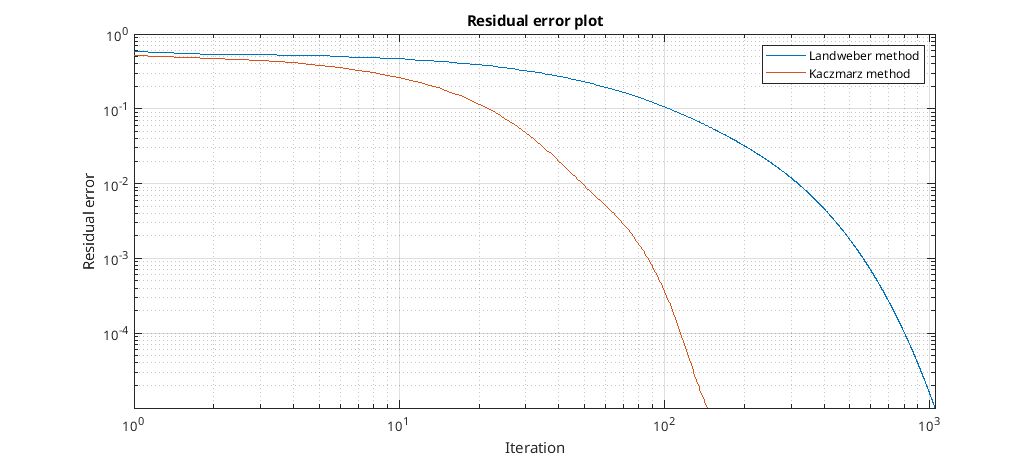
\includegraphics[width=1\textwidth]{images/Residuals_Problem2.png}
    \caption{Residuals of Kaczmarz and Landweber methods}
\end{figure}
\begin{figure}[H]
  \centering
  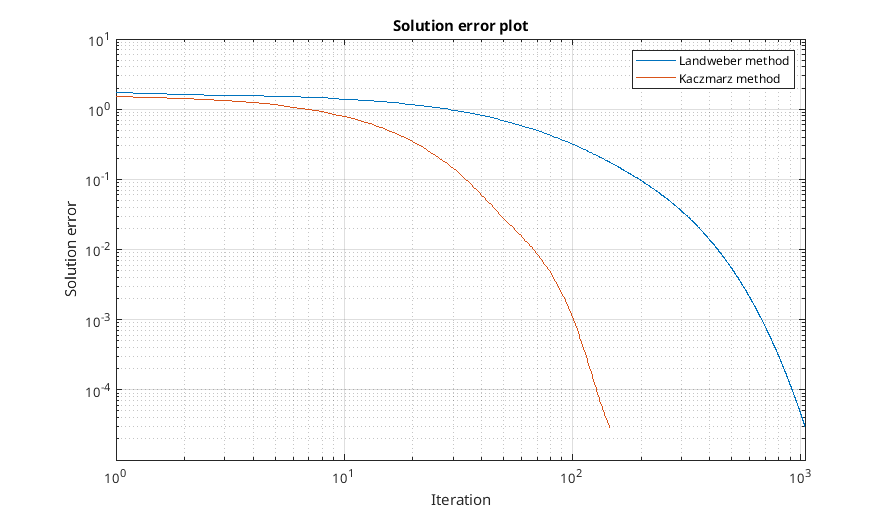
\includegraphics[width=1\textwidth]{images/Solution_Problem2.png}
  \caption{Solution errors of Kaczmarz and Landweber methods}
\end{figure}